\chapter{L'endoparasitoïdisme favorise l'endogénisation et la domestication des virus à dsDNA}

Le transfert de gènes entre organismes non apparentés a été découvert comme une source importante d'innovation génétique, qui peut parfois aboutir à de l'adaptation. Ces transferts horizontaux de gènes (THG) sont courants chez les procaryotes, et leurs effets sont reconnus depuis longtemps. Des travaux récents suggèrent que les eucaryotes peuvent également être engagés dans ces processus \citep{irwin_systematic_2022}. Cependant, les paramètres qui déterminent la structure des THGs impliquant des eucaryotes restent inconnus.\\

Dans cette étude, nous faisons l'hypothèse que le mode de vie des Hyménoptères est un facteur structurant les chances d'endogénisation des gènes viraux. Plusieurs séries d’études documentant des évènements de domestications de machineries virales entières exclusivement par des guêpes endoparasitoïdes ont motivé cette hypothèse. Dans tous les cas décrits, des structures de type virales codées par des gènes de virus à dsDNA permettent d’adresser des facteurs de virulence qui protègent les progéniteurs des guêpes du système immunitaire de leur hôte \citep{bezier_polydnaviruses_2009,volkoff_analysis_2010,burke_common_2019,pichon_recurrent_2015,di_giovanni_behavior-manipulating_2020}. \\

À partir de ces données, notre hypothèse de travail est que le mode de vie endoparasitoïde peut être associé à un taux plus élevé d'endogénisation virale et/ou à un taux plus élevé d'événements de domestication, pour deux raisons non exclusives impliquant (i) l'exposition à de nombreux virus et/ou (ii) la valeur adaptative des éléments endogénisés.\\

Selon le premier argument, un taux plus élevé d'endogénisation peut provenir d'une exposition accrue aux virus. En raison de l'interaction intime entre l'œuf ou la larve d'un endoparasitoïde et son hôte, cet effet pourrait être particulièrement présent chez les endoparasitoïdes. En d'autres termes, l'endoparasitoïsme pourrait faciliter l'acquisition de nouveaux virus auprès des hôtes, ainsi que le maintien et la propagation des virus nouvellement acquis au sein des populations de guêpes, en raison de leur mode de vie unique. En effet, les guêpes endoparasitoïdes injectent fréquemment non seulement des œufs mais aussi du venin (généralement produit dans la glande à venin ou les cellules du calice) où peuvent se loger des virus, profitant ainsi d'une transmission verticale, facilitant ainsi leur propagation verticale \citep{martinez_additional_2016,coffman_viral_2022}. De plus, le confinement de plusieurs guêpes en développement au sein d'un seul hôte peut faciliter la transmission horizontale du virus et la propagation ultérieure de la population parmi les guêpes (par exemple, \citep{varaldi_infectious_2003,coffman_viral_2022}).\\

Selon le second argument, les insertions virales et le taux de domestication serait plus élevés chez les endoparasitoïdes car leur endogénization aurait été sélectionnée positivement. En effet, contrairement à d'autres modes de vie, échapper au système immunitaire de l'hôte est particulièrement difficile à relever pour ces insectes comparés à d'autres Hyménoptères au style de vie ectoparasitoïde par exemple, pour lesquels les progénitures ne sont pas en interaction étroite avec le système immunitaire de l'hôte. Cette pression sélective peut donc favoriser la cooptation de caractéristiques virales, telles que l'activité de fusion membranaire des virus, ce qui peut optimiser la délivrance des facteurs de virulence.\\

Pour tester ces hypothèses, un pipeline bioinformatique a été construit afin de rechercher des EVEs dans des génomes. Celui-ci comporte trois étapes principales. i : la recherche systématique d'éléments viraux endogènes par homologie de séquence avec une base de données exhaustive de protéines virales, ainsi que des indices permettant de tester l'hypothèse d'endogénisation, telles que la couverture de séquençage le long des scaffolds contenant des EVEs ou la proximité avec d'autres éléments génétiques eucaryotes typiques. ii: l'examen de l'histoire évolutive des insertions, qui est comparée à la phylogénie des espèces. Et enfin, iii, l'investigation systématique, si possible, du caractère adaptatif de ces insertions en étudiant le régime de sélection des séquences depuis leur endogénisation par des approches de \textit{dN/dS} ou par l'analyse des profils d'expression. \\

Nous avons appliqué ce pipeline à 124 espèces d'hyménoptères (dont 32 correspondaient à des génomes de parasitoïdes séquencés par le laboratoire). Ces résultats ont permis de découvrir plusieurs nouveaux cas d'endogénisation et de domestication de virus chez les Hyménoptères. Nous montrons dans un premier temps que les virus à dsDNA sont beaucoup plus souvent endogénisés et domestiqués qu'attendu selon la répartition de ces virus chez les insectes (\figurename{\ref{figure:Resume_figure_papier1_1}}).\\

\begin{figure}[!htpbt]
\captionsetup{font=footnotesize}
 \centering
  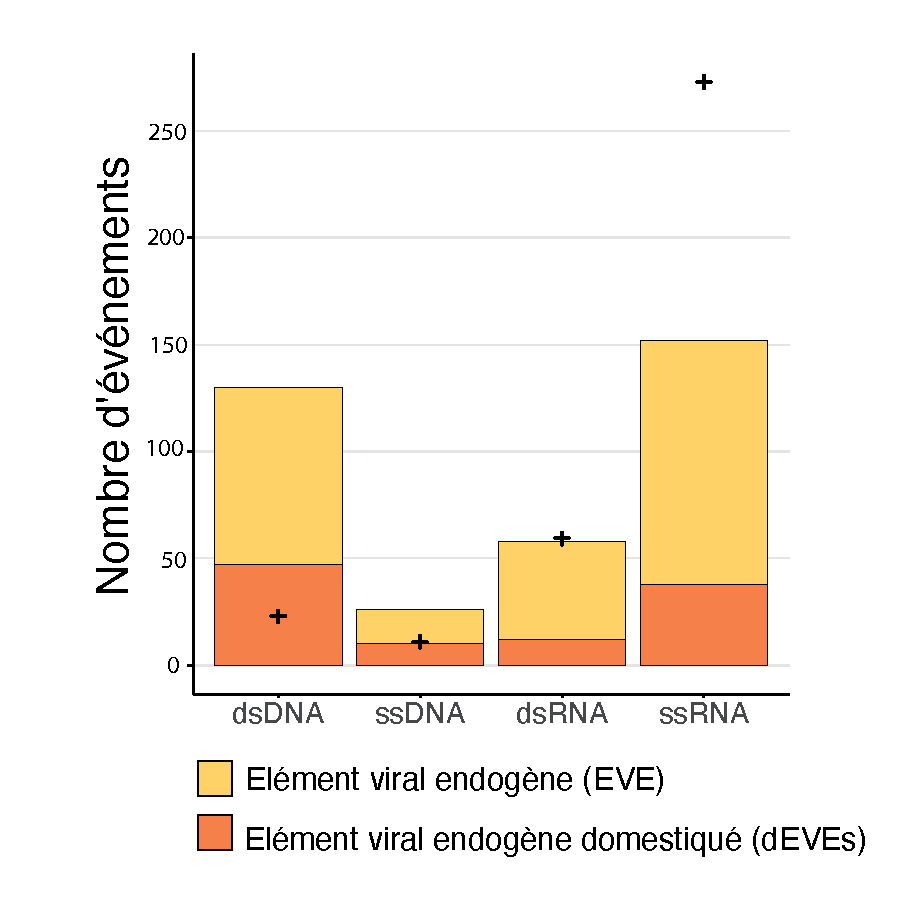
\includegraphics[width=\linewidth,height=\textheight,keepaspectratio]{PhD-master/figures/Resume_figure_papier1_1.pdf}
\caption[Paper1:Figures principales récapitulatives du chapitre1\_1]{\textbf{Distribution des évènements en fonction des structures génomiques}. Distribution du nombre d'événements inférés, selon les quatre catégories de structures génomiques virales. Les croix renvoient au nombre attendu d'événements d'endogénisation pour chaque catégorie en fonction de leur abondance relative estimée chez les insectes en s'appuyant sur les séquences disponibles dans les bases de données (voir les détails dans \hyperref[sec:MM-8]{Matériel et méthodes} et les données sur les virus infectés dans le fichier GitHub : \href{https://github.com/BenjaminGuinet/PhD_defense/blob/main/Supplementary_paper1/All_virus_infecting_insects_informations.csv}{All\_virus\_infecting\_insects\_informations.csv}.}
\label{figure:Resume_figure_papier1_1}
\end{figure}

Pour expliquer ce phénomène, nous pouvons supposer que la prévalence observée des virus à dsDNA est le résultat d'un potentiel de transfert de matériel adaptatif plus important que celui des autres virus (\figurename{\ref{figure:Resume_figure_papier1_1}}). En effet, nous pourrions imaginer que les virus à ADN double brins seraient plus à même à rentrer dans les génomes que les hôtes compte tenu du fait qu'ils présentent des génomes de même structure que ceux des guêpes et que la plupart se répliquent dans le noyau de leurs hôtes. En effet, la réplication nucléaire est une caractéristique partagée par presque toutes les familles de virus à dsDNA trouvées dans notre analyse : \textit{Baculoviridae}, \textit{Iridoviridae}, \textit{Phycodnaviridae}, \textit{Nimaviridae}. \textit{Caulimoviridae}, \textit{Herpesviridae}, \textit{Asfaviridae} \citep{schmid_dna_2014,harrison_ictv_2020,international_committee_on_taxonomy_of_viruses_virus_2012,teycheney_ictv_2020,verbruggen_molecular_2016}, les virus filamenteux d'\textit{Apis mallifera} (AmFV) \citep{clark_filamentous_1978} et le virus filamenteux LbFV \citep{varaldi_artifical_2006} (les \textit{Poxviridae}, qui se répliquent dans le cytoplasme, sont donc la seule exception). \\

\begin{figure}[H]
\captionsetup{font=footnotesize}
 \centering
  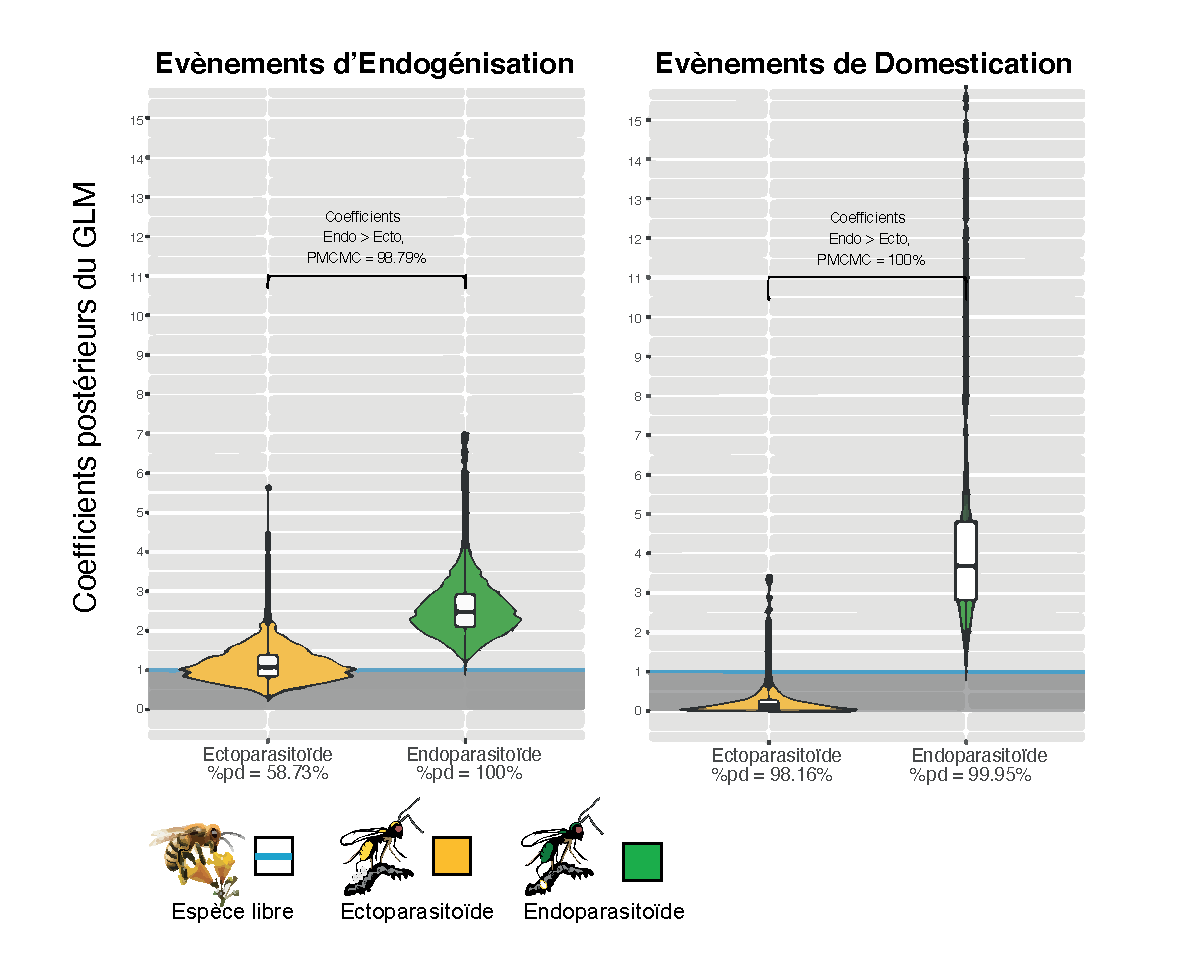
\includegraphics[width=\linewidth,height=\textheight,keepaspectratio]{PhD-master/figures/Resume_figure_papier1_2.pdf}
\caption[Paper1:Figures principales récapitulatives du chapitre1\_2]{\textbf{Distribution des coefficients de taux d'endogénisation et de domestication de virus à dsDNA selon les styles de vie}. Les diagrammes en violon représentent la distribution postérieure des coefficients d'évènements impliquant des virus à dsDNA obtenus sous les différents modèles GLM (après transformation exponentielle pour obtenir un taux relatif aux espèces libres). Les coefficients sont dérivés de 1000 modèles GLM indépendants, où 1000 scénarios probables d'états ancestraux aux nœuds ont été échantillonnés de manière aléatoire parmi les itérations MCMCM (voir les détails dans \hyperref[sec:MM-12]{Matériel et méthodes}). Le \%pd est la probabilité de direction et indique la proportion de la distribution postérieure où les coefficients ont le même signe que le coefficient médian. Le $P_{MCMCM}$ indique la proportion d'itérations MCMC où le coefficient obtenu pour les espèces endoparasitoïdes est plus élevé que pour les espèces ectoparasitoïdes. Tous les résumés statistiques des modèles GLM bayésiens peuvent être trouvés sur le dépôt GitHub sous le nom : \href{https://github.com/BenjaminGuinet/PhD_defense/blob/main/Supplementary_paper1/Lifestyle_statistical_analysis_results.xlsx}{Lifestyle\_statistical\_analysis\_results.xlsx}.}
\label{figure:Resume_figure_papier1_2}
\end{figure}

.\newline
Enfin, nous apportons également des arguments que les guêpes endoparasitoïdes sont plus susceptibles que les ectoparasitoïdes et les espèces libres d'endogéniser et de domestiquer les virus à ADN double brin (\figurename{\ref{figure:Resume_figure_papier1_2}}).\\

Nous pouvons alors essayer de comprendre pourquoi les guêpes endoparasitoïdes subiraient des évènements d'endogénisation plus fréquemment que les espèces libres ou au style de vie ectoparasitoïde. Selon notre première hypothèse, selon laquelle les endoparasitoïdes peuvent présenter plus d'événements d'endogénisation parce qu'ils interagissent avec plus de virus, nous nous attendions que tous les virus, quelle que soit leur structure génétique, bénéficient de cet effet. En particulier, nous devrions observer cet effet chez les virus à ARN, qui sont impliqués dans le plus grand nombre d'événements d'endogénisation. Cependant, seuls les virus à dsDNA présentaient des profils d’endogénisation et de domestication beaucoup plus fréquents que les autres styles de vie. Par conséquent, nous pensons que cette explication est peu probable. \\

Notre deuxième hypothèse était que les endoparasitoïdes seraient sélectionnés pour maintenir des gènes d'origine virale, car leur rétention améliorerait leur valeur selective dans un contexte immunitaire. Dans nos résultats, les événements de domestication sont plus fréquemment observés chez les endoparasitoïdes (plus de 3 fois plus d'évènements que chez les autres Hyménoptères) (\figurename{\ref{figure:Resume_figure_papier1_2}}). Il est clair qu'une partie de ce phénomène peut s'expliquer par l'apport accru indiqué ci-dessus (le taux plus élevé d'endogénisation). Après avoir contrôlé ce facteur, une tendance vers un taux de domestication plus élevé persiste. Plus précisément, la probabilité de domestication après endogénisation était considérablement plus élevée pour les endoparasitoïdes que pour les ectoparasitoïdes, mais pas significativement plus élevée que pour les espèces libres. Cependant, si un seul événement de domestication empêche la domestication d'autres EVE sans affecter le taux d'endogénisation non adaptative, alors on s'attend à de très faibles différences sur cet indice. En effet, cet effet entrainerait la "dilution" du signal lié à la domestication le long des branches. Si cet effet est en jeu, alors notre capacité à détecter toute différence dans les taux de domestication entre les modes de vie est considérablement réduite.\\

Enfin, si les virus à dsDNA sont plus susceptibles d'être domestiqués par les guêpes endoparasitoïdes, c'est peut-être parce que leurs structures génomiques virales sont similaires à celles des guêpes, ce qui les rendrait plus simples à assimiler pour les génomes. De plus, d'autres propriétés des virus à ADN double brin peuvent expliquer ce pattern. En effet, L'ADN qui est emballé dans les particules matures code généralement des protéines de virulence provenant de la guêpe \citep{espagne_genome_2004}. Cela signifie que, au moins pour ces cas, le système viral devrait être capable d'emballer l'ADN, ce qui est très probablement une caractéristique que les virus à ADN peuvent fournir. Cet argument ne tient pas dans les systèmes VLPs, où seules les protéines sont emballées dans les particules virales, et on ne voit pas pourquoi les EVE dérivées de virus à dsDNA seraient plus à même de remplir une telle fonction. D'autres caractéristiques des virus à dsDNA apparaissent ici comme des facteurs potentiellement importants : la grande taille de leur génome et la taille de leur capside et de leur enveloppe \citep{chaudhari_scaling_2021}. Ces caractéristiques pourraient prédisposer les virus à dsDNA à être domestiqués, puisque d'abondantes quantités de venins doivent être transmises afin de supprimer efficacement la réponse immunitaire de l'hôte.\\

En conclusion, nous faisons l'hypothèse que les taux plus élevé d'endogénisation et le plus grand nombre d'événements de domestication de virus dsDNA chez les endoparasitoïdes sont le résultat de l'intense pression sélective exercée par le système immunitaire de l'hôte sur les endoparasitoïdes. Cette pression sélective sévère peut favoriser les endoparasitoïdes qui conservent une machinerie virale qui les aide à s'attaquer aux facteurs de virulence de leurs hôtes. Plus largement, nous estimons que ce phénomène devrait être omniprésent chez les espèces d'insectes ayant un mode de vie similaire.\\


Le manuscrit est actuellement en review dans le journal eLife et est disponible sous forme de preprint sur \href{https://doi.org/10.1101/2022.11.16.515002}{bioRxiv} sous le DOI : 10.1101/2022.11.16.515002.\\

Ces travaux sont également disponibles en anglais reformaté dans la première section du chapitre \hyperref[sec:chap1]{Études}. 
